\documentclass[11pt,letterpaper]{article}
\usepackage[T1]{fontenc}
\usepackage[utf8]{inputenc}
\usepackage{lmodern}
\usepackage[margin=1in,headheight=14pt]{geometry}
\usepackage{amsmath,amssymb,amsthm,mathtools}
\usepackage{microtype,booktabs,longtable,tabularx,array,graphicx}
\usepackage{xcolor,enumitem,fancyhdr,xurl}
\definecolor{ink}{HTML}{17334A}
\definecolor{accent}{HTML}{197A84}
\definecolor{light}{HTML}{EDF3F6}
\usepackage[colorlinks=true,linkcolor=ink,urlcolor=accent,citecolor=ink,
  pdftitle={Beyond Dirichlet GRH: transfer mechanisms and exact obstructions},
  pdfauthor={Research analysis prepared for Vladimir Reshetnikov}]{hyperref}
\usepackage{titlesec}
\titleformat{\section}{\large\sffamily\bfseries\color{ink}}{\thesection}{.7em}{}
\titleformat{\subsection}{\normalsize\sffamily\bfseries\color{ink}}{\thesubsection}{.7em}{}
\newtheorem{theorem}{Theorem}[section]
\newtheorem{lemma}[theorem]{Lemma}
\newtheorem{proposition}[theorem]{Proposition}
\newtheorem{corollary}[theorem]{Corollary}
\theoremstyle{definition}
\newtheorem{definition}[theorem]{Definition}
\theoremstyle{remark}
\newtheorem{remark}[theorem]{Remark}
\newcommand{\Q}{\mathbb Q}
\newcommand{\R}{\mathbb R}
\newcommand{\C}{\mathbb C}
\newcommand{\Z}{\mathbb Z}
\DeclareMathOperator{\Gal}{Gal}
\DeclareMathOperator{\Frob}{Frob}
\DeclareMathOperator{\RH}{RH}
\setlist{itemsep=3pt,topsep=5pt}
\setlength{\emergencystretch}{3em}
\pagestyle{fancy}
\fancyhf{}
\fancyhead[L]{\small\sffamily Beyond Dirichlet GRH}
\fancyhead[R]{\small\sffamily Transfer analysis}
\fancyfoot[C]{\small\thepage}
\renewcommand{\headrulewidth}{.3pt}
\begin{document}
\begin{titlepage}
\vspace*{.45in}
{\sffamily\color{accent}\large RESEARCH REPORT\par}
\vspace{.22in}
{\sffamily\bfseries\color{ink}\Huge Beyond Dirichlet GRH\par}
\vspace{.18in}
{\sffamily\LARGE Transfer mechanisms, exact obstructions,\\[5pt]
and a concrete cubic target\par}
\vspace{.35in}
{\large Prepared for Vladimir Reshetnikov\par}
\vspace{.08in}
{November 25, 2026\par}
\vspace{.4in}
\noindent\colorbox{light}{\begin{minipage}{.94\textwidth}
\vspace{9pt}
\textbf{Result.} The proof contains reusable arithmetic machinery, but this
analysis does not establish another open conjecture. It supplies three
precise advances beyond the earlier reports: an optimal fixed-congruence
approximation theorem for every finite Galois group; a sharp interpolation
and finite-sum reduction for nonabelian Dedekind RH; and a ramification
constraint explaining why arbitrarily small normalized Selmer lengths do
not by themselves imply vanishing.
\vspace{7pt}

\textbf{Recommended first target.} Prove one explicit upper bound for
root counts of $T^3-T-1$ modulo primes. Its validity at all fourth-power
scales is equivalent to RH for the associated cubic field. The missing
step is a class-sensitive arithmetic estimate.
\vspace{9pt}
\end{minipage}}
\vfill
\noindent\textbf{Upstream snapshot}\par
\path{lsernau/grh-lean}\par
\path{72fead102f663d5c7a407964a13dc0cf9d977207}\par
\vspace{8pt}
\noindent All 1,627 tracked file blobs match the GitHub inventory. The six
earlier incoming archives were resolved by exact blob hashes. This is a
source-level analysis, not a new full Lean build or kernel replay.
\end{titlepage}

\tableofcontents
\newpage

\section{Assessment and scope}

\subsection{The answer to the research question}

There is a credible route from the repository's \emph{method} to further
questions. The strongest immediate candidate is RH for a fixed nonabelian
number field. The central construction combines many short integral
automorphic forms with a lower bound for their determinant. Its output is
a one-sided inequality for a positive weighted prime sum. The analytic
conversion of such an inequality into a zero-free half-plane extends
well beyond Dirichlet characters. What does not automatically extend is
the arithmetic realization of the new prime weights.

The word GRH needs an exact scope here. The five exported statements in
\path{grh/src/Main.lean}, whose types are fixed in
\path{grh/src/Statements.lean}, prove RH for the Riemann zeta function and
GRH for \emph{Dirichlet} $L$-functions. This includes all positive moduli
and imprimitive characters, with the stated exception at the principal
character's pole. The files do not state RH for arbitrary Dedekind,
Hecke, Artin, or automorphic $L$-functions. We take the exported theorem
as available, as requested, and investigate extensions of its proof.
\cite{grh-main,grh-statements}

This report does not obtain a new famous-conjecture solution. It does
identify exact mathematical work that would constitute such a solution,
prove reusable refinements, and rule out two tempting shortcuts. That
distinction matters: replacing a conjecture by an equivalent estimate is
a useful research specification, but the estimate still needs proof.

\subsection{The principal findings}

\begin{enumerate}
\item \textbf{Fixed congruences lose exactly the nonabelian character
information.} If $\chi$ is a nonlinear irreducible character of a finite
Galois group and $a$ is any function of $p$ modulo a fixed $q$, then
\[
 \lim_{X\to\infty}\frac1{\pi(X)}\sum_{p\le X}
  |\chi(\Frob_p)-a(p\bmod q)|^2
 =1+\frac1{\varphi(q)}\sum_{b\in(\Z/q\Z)^\times}|a(b)|^2.
\]
The finite omitted set consists of ramified primes and primes dividing
$q$. This sharpens the previous cubic obstruction to every finite Galois
group and gives the optimal approximation for arbitrary class functions.

\item \textbf{The nonabelian analytic target admits explicit finite sums
and sparse scales.} Let $f$ be any monic irreducible integer polynomial,
$K=\Q[T]/(f)$, and $r_f(p)$ its number of roots modulo $p$. Put
\[
 S_f(x)=\sum_{\substack{p\le x\\p\nmid\operatorname{disc}(f)}}
 r_f(p)\log p\left(\frac1p-\frac1x\right),\qquad
 B_f(n)=\log16-S_f(16n^4)+S_f(n^4).
\]
Then
\begin{equation}\label{eq:headline-target}
 \boxed{\quad \RH(\zeta_K)\ \Longleftrightarrow\
                  \sup_{n\ge1}n^2B_f(n)<\infty.\quad}
\end{equation}
Every individual $B_f(n)$ is a finite expression. There is no unknown
Euler--Kronecker constant in it. The theorem still quantifies over
\emph{all} $n$; a finite computation cannot prove its right-hand side.

\item \textbf{The Selmer error budget has a compulsory ramification
cost.} If all first $m$ powers of an $\ell$-power-order auxiliary
character satisfy a local budget $\varepsilon$ on $Q\cup\overline Q$,
with $Q\ne\varnothing$, and its values lie in a coefficient ring of
ramification index $e$, then
\[
       \varepsilon e\ge 2|Q|\ell^{\lfloor\log_\ell m\rfloor}.
\]
Normalized length has mesh $1/e$, so even a zero fixed term in the
Selmer bound does not make this error small enough to certify vanishing
by integer rounding. The source also contains a useful positive
refinement: the \emph{number} of auxiliary ramification pairs can be
bounded independently of $m$ and $\varepsilon$.
\end{enumerate}

The first result uses classical representation theory and Chebotarev;
the third is elementary local valuation theory applied to the source.
The fourth-power sampling scale in the second result already appears
in a November 2026 preprint, and the exact logarithmic interpolation
constant is the classical Specht ratio. We provide complete derivations
and the nonabelian specialization, without claiming priority.
\cite{milne,setiawan,specht}

\subsection{What was inspected and checked}

The inspected upstream commit is
\path{72fead102f663d5c7a407964a13dc0cf9d977207}. Its readable edition
contains 803 Lean source files; the compact edition contains 794.
All 1,627 tracked file blobs in the local snapshot matched the returned
GitHub tree inventory, and the working tree was clean. The pinned
toolchain is Lean 4.35.0, with Mathlib commit
\path{56a005855ea17e0b0958f73ec801ae140b0a1679}.

The repository reports compilation, standard-axiom checks, and independent
checker runs. Those are upstream reports. This session inspected the
endpoint statements and the relevant analytic, determinant, and Selmer
proofs; it did not repeat the complete compilation or kernel checks.
The delivered Lean file is an interface specification and audit driver,
explicitly marked uncompiled. The mathematical arguments in this report
are human-readable proofs, not claims of new Lean formalizations.
\cite{grh-readme}

\section{Relationship to the six earlier reports}

The incoming directory at ProveIt commit
\path{13c30b3b677b691845466289bfdb792d11fefad5} contains six relevant
archives. Their complete blob identifiers and sizes are recorded in
\path{evidence/provenance.json}. The earlier reports already do much of
the broad survey work; this analysis uses that foundation rather than
presenting their conditional reductions as new solutions.

\begin{longtable}{@{}p{.37\textwidth}p{.58\textwidth}@{}}
\toprule
Archive & Material already present \\
\midrule
\endhead
\path{grh_transfer_analysis.zip} &
Quantitative determinant comparison, a one-sided analytic criterion,
and the cubic field of discriminant $-23$ with its principal-ideal
selector and missing arithmetic realization.\\[5pt]
\path{grh_transfer_analysis_2026-11-25.zip} &
Sparse successful-twist hypotheses, the pure Tate-twist obstruction,
and careful separation of products from gcds in Hecke certificates.\\[5pt]
\path{grh_lean_transfer_analysis.zip} &
An overlapping audit and the four arithmetic requirements for the
cubic transfer; no completed cubic RH estimate.\\[5pt]
\path{grh-transfer.zip} &
Completely split-prime criteria for general finite Galois fields,
limsup information, and several arithmetic classification applications.\\[5pt]
\path{grh_transfers.zip} &
Exponent-six class-group restrictions, fixed-window prime-race
criteria, and a degree-two character obstruction.\\[5pt]
\path{grh-lean-transfers.zip} &
CM genus-field containment, proposed prime-degree coefficient-field
classifications, and additional prime-race and cubic results.\\
\bottomrule
\end{longtable}

The present report does not independently recertify every classification
claimed in those packages. The comparison distinguishes their proved
lemmas, stated classifications, and unresolved transfer targets. In
particular, a familiar conditional theorem becoming unconditional after
Dirichlet GRH is not counted here as a new application of the proof
mechanism. The relevant CM finiteness program is already developed in
Martin's work and the earlier reports.\cite{martin}

The additions here are the exact conditional-expectation formula in
Section~\ref{sec:periodic-obstruction}, the generalized and explicitly
centered finite-sum specification in Section~\ref{sec:sparse-sampling},
and the ramification/discreteness analysis in
Section~\ref{sec:ramification-budget}. These improve the precision of
the next research step. They do not silently upgrade an earlier
conditional statement to an unconditional one.

\section{What actually makes the proof work}

\subsection{A positive arithmetic statistic}

For a suitable auxiliary imaginary quadratic field with character
$\chi_d$, the source studies
\[
 \lambda_{d,q}(n)=\Lambda(n)(1-\chi_d(n))\mathbf 1_{n\equiv1\pmod q},
 \qquad
 R_{d,q}(x)=\sum_{n\le x}\lambda_{d,q}(n)
       \left(\frac1n-\frac1x\right)-\frac{\log x}{\varphi(q)}-c_{d,q}.
\]
These coefficients are nonnegative. The analytic transform records a
difference of logarithmic derivatives of original and quadratic-twisted
Dirichlet functions. A carefully chosen auxiliary twist avoids
cancellation at a proposed zero. Landau's positivity principle then
converts an eventual one-sided upper bound into nonvanishing.
The actual statement has quantified hypotheses over suitable auxiliary
primes; one should not replace it by a generic slogan that any signed
prime sum detects zeros.\cite{criterion,prime-sums}

\subsection{The short, numerous, and long-form comparison}

The arithmetic part compares the same covolume corrected by its index
from two sides. Schematically, for a target of dimension $d$, $n$
independent constructed forms, and $W=(V+2\delta)/d$,
\[
 H-E_{\rm lower}\le W
 \le H-\frac nd\,m\mathcal R+E_{\rm upper},
 \qquad n\ge d/2.
\]
Here $d>0$, the two $E$ terms are nonnegative errors,
$H$ is a shared main term, $V$ a logarithmic squared covolume,
$\delta$ an integral-index cost, $m$ the chain length, and
$\mathcal R$ an arithmetic remainder. Cancellation of $H$ gives
\[
 m\mathcal R\le\frac dn(E_{\rm lower}+E_{\rm upper})
       \le2(E_{\rm lower}+E_{\rm upper}).
\]
The elementary cancellation is not the difficult theorem. The hard
content is producing the forms, preserving a sufficiently large
independent family, controlling all denominators, and making the
archimedean and nonarchimedean main terms agree.

In the source this becomes
\[
 D.m\,D.totalRemainder\le D.f\,D.a\,(\log b)^5.
\]
After translating the total remainder back into prime sums,
\begin{align*}
 R_{d,q}(x)\le {}&\frac{\varphi(q)(\log b)^6}{m}
       +|R_{d,q}(x_1)|+(\log b)|R_{d,1}(x_1)|.
\end{align*}
One chooses $m\asymp\sqrt x$, lets $\log b$ grow sufficiently slowly
relative to powers of $x$, and sends the comparison cutoff $x_1$ very
far out. The prime number theorem at $x_1$ then makes the last two terms
small. This is why a square-root exponent appears. It is not obtained
merely by applying a stronger version of Chebyshev's inequality.
\cite{main-inequality,one-sided}

\subsection{Which parts are portable}

\begin{longtable}{@{}p{.27\textwidth}p{.31\textwidth}p{.35\textwidth}@{}}
\toprule
Ingredient & Portable content & New work for a nonabelian target\\
\midrule
\endhead
One-sided Landau argument &
Meromorphic continuation, residue signs, and a positive barrier &
Identify a transform whose poles cannot cancel the desired zeros.\\[5pt]
Integral determinant comparison &
One index-corrected determinant with matching upper/lower main terms &
Construct the target forms and preserve all quantitative losses.\\[5pt]
Prime divisibility &
Local valuations encode a positive prime statistic &
Make the valuations distinguish Frobenius classes beyond their abelian image.\\[5pt]
Auxiliary twisting &
Simultaneous control of finite collections and powers at one coefficient prime &
Supply a valid comparison to the fixed arithmetic object of interest.\\[5pt]
Scale selection &
Sparse checkpoints can be sufficient for the analytic conclusion &
Prove estimates at infinitely many prescribed checkpoints, with uniform constants.\\
\bottomrule
\end{longtable}

The twisting quantifier is especially consequential: favorable characters
can be chosen separately at different coefficient primes and embeddings.
That is exactly what the determinant-height argument needs. It does not
give a single global twist with every desired local property. Similarly,
the fixed-modulus constants in the existing construction do not furnish
the growing-modulus uniformity needed for Elliott--Halberstam-type
questions. These are substantive mathematical requirements, not
formalization bookkeeping.

% Fragment for inclusion in the main report.
% Requires amsmath, amssymb, amsthm and theorem/corollary environments.
\section{The exact information lost by fixed congruence weights}
\label{sec:periodic-obstruction}

The earlier reports establish a mean-square obstruction for the standard
character of an $S_3$ cubic field. The same obstruction holds for every
nonlinear irreducible character of every finite Galois group. More generally,
one can compute the optimal periodic approximation to any Frobenius class
function exactly. This is an application of character theory and the classical
Chebotarev theorem; it is a diagnostic for proposed extensions, not a claim
to solve another open conjecture.

Let $M/\mathbb Q$ be a finite Galois extension with group $G$. Fix an integer
$q\ge1$ and put
\[
 A_q=(\mathbb Z/q\mathbb Z)^\times,\qquad
 E_q=M\cap\mathbb Q(\zeta_q),\qquad
 H_q=\operatorname{Gal}(M/E_q).
\]
For $q=1$, interpret $A_q$ as the trivial group. Since $E_q/\mathbb Q$ is
abelian, $H_q$ is normal and contains the commutator subgroup $[G,G]$.
Let $S$ be any fixed finite set containing the primes ramifying in $M$ and
the primes dividing $q$. At every $p\notin S$, choose a representative
$g_p\in G$ of the arithmetic Frobenius conjugacy class. If $f:G\to\mathbb C$ is a class
function, its value $f(g_p)$ is independent of this choice.

The restriction of $b\in A_q=\operatorname{Gal}(\mathbb Q(\zeta_q)/\mathbb Q)$
to $E_q$ determines one coset of $H_q$ in $G$. Define
\begin{equation}\label{eq:periodic-best}
 m_q(b)=\frac1{|H_q|}
   \sum_{\substack{g\in G\\g|_{E_q}=b|_{E_q}}}f(g).
\end{equation}
Thus $m_q$ is a finite, explicitly specified function on the reduced residue
classes. Write
\[
 \|f\|_G^2=\frac1{|G|}\sum_{g\in G}|f(g)|^2,
 \qquad
 \|a\|_{A_q}^2=\frac1{\varphi(q)}\sum_{b\in A_q}|a(b)|^2.
\]

\begin{theorem}[Optimal approximation by a fixed modulus]
\label{thm:periodic-projection}
For every class function $f:G\to\mathbb C$ and every function
$a:A_q\to\mathbb C$, both of the following limits exist and have the same
value:
\begin{align}
 \lim_{X\to\infty}\frac1{\pi(X)}
   \sum_{\substack{p\le X\\p\notin S}}
       |f(g_p)-a(p\bmod q)|^2
 &\;=\;\mathcal E_q(f,a),\label{eq:unweighted-mse}\\
 \lim_{X\to\infty}\frac1X
   \sum_{\substack{p\le X\\p\notin S}}
       (\log p)|f(g_p)-a(p\bmod q)|^2
 &\;=\;\mathcal E_q(f,a),\label{eq:weighted-mse}
 \intertext{where}
 \mathcal E_q(f,a)
 &=\|f\|_G^2-\|m_q\|_{A_q}^2
                  +\|a-m_q\|_{A_q}^2.\label{eq:mse-decomposition}
\end{align}
Consequently $m_q$ is the unique optimal approximation on $A_q$, and the
minimum error is $\|f\|_G^2-\|m_q\|_{A_q}^2$.

Let $f=\sum_{\chi\in\operatorname{Irr}(G)}c_\chi\chi$ be its expansion in
irreducible characters, with the usual normalized character inner product.
Then the minimum has the equivalent expression
\begin{equation}\label{eq:mse-character-energy}
 \min_a\mathcal E_q(f,a)
 =\sum_{\substack{\chi\in\operatorname{Irr}(G)\\
                    H_q\not\subseteq\ker\chi}}|c_\chi|^2.
\end{equation}
Here $H_q\subseteq\ker\chi$ means that the representation affording
$\chi$ is trivial on $H_q$.
\end{theorem}

\begin{proof}
Put $N=M\mathbb Q(\zeta_q)$. Restriction identifies its Galois group with
the fiber product
\[
 \Gamma=\{(g,b)\in G\times A_q:
                  g|_{E_q}=b|_{E_q}\}.
\]
Its projection onto $A_q$ is surjective and has fibers of size $|H_q|$,
so $|\Gamma|=\varphi(q)|H_q|$. The function
$F(g,b)=|f(g)-a(b)|^2$ is constant on conjugacy classes of $\Gamma$:
$f$ is a class function and $A_q$ is abelian. Chebotarev's density theorem,
summed over the finitely many conjugacy classes, gives
\begin{equation}\label{eq:fiber-product-average}
 \lim_{X\to\infty}\frac1{\pi(X)}
    \sum_{\substack{p\le X\\p\notin S}}F(g_p,p\bmod q)
 =\frac1{\varphi(q)|H_q|}
    \sum_{b\in A_q}
    \sum_{g|_{E_q}=b|_{E_q}}|f(g)-a(b)|^2.
\end{equation}
This is the unconditional fixed-field Chebotarev theorem. No GRH, effective
error estimate, or uniformity in $M$ or $q$ is being used.

For a fixed $b$, the mean of $f$ over the indicated coset is $m_q(b)$.
Expanding the square and using the vanishing of the mean of $f-m_q(b)$
on that coset gives the orthogonal decomposition
\[
 \frac1{|H_q|}\sum_{g|_{E_q}=b|_{E_q}}|f(g)-a(b)|^2
 =\frac1{|H_q|}\sum_{g|_{E_q}=b|_{E_q}}|f(g)-m_q(b)|^2
      +|m_q(b)-a(b)|^2.
\]
Average over $b$. Every $g\in G$ is counted the same number of times,
because the restriction $A_q\to\operatorname{Gal}(E_q/\mathbb Q)$ is
surjective. This proves \eqref{eq:mse-decomposition} and uniqueness of the
minimum, since every residue class has the positive weight
$1/\varphi(q)$.

For completeness the logarithmic prime weight does not change the limit.
Write $U(X)$ for the unweighted numerator in
\eqref{eq:unweighted-mse}. Chebotarev and the ordinary prime number theorem
give
$U(X)=\mathcal E_q(f,a)\operatorname{Li}(X)+o(X/\log X)$.
Partial summation yields
\[
 \sum_{\substack{p\le X\\p\notin S}}(\log p)F(g_p,p\bmod q)
 =U(X)\log X-\int_2^X\frac{U(t)}t\,dt
 =\mathcal E_q(f,a)X+o(X).
\]
Changing the fixed lower endpoint alters only a constant. This proves
\eqref{eq:weighted-mse}. Equivalently one may normalize the two sums by
the number of retained primes and by their sum of logarithms, respectively:
those denominators are asymptotic to $\pi(X)$ and $X$. Deleting or adding
finitely many unramified primes does not affect either limit.

It remains to identify the character components retained by the coset
average. Let $\rho$ be an irreducible representation of $G$ with character
$\chi$, and set
\[
 P_H=\frac1{|H_q|}\sum_{h\in H_q}\rho(h).
\]
This is projection onto the subspace fixed by $H_q$. Because $H_q$ is
normal, that subspace is $G$-invariant; by irreducibility it is either
zero or the whole representation. Therefore
\[
 \frac1{|H_q|}\sum_{h\in H_q}\chi(gh)
 =\operatorname{tr}(\rho(g)P_H)
 =\begin{cases}
   \chi(g),&H_q\subseteq\ker\chi,\\
   0,&H_q\not\subseteq\ker\chi.
  \end{cases}
\]
The characters in the first case factor through the abelian quotient
$G/H_q$ and hence have degree one. Irreducible-character orthogonality
now makes the squared norm lost by this projection exactly the sum in
\eqref{eq:mse-character-energy}.
\end{proof}

\begin{corollary}[Every nonlinear irreducible trace is invisible to fixed congruences]
\label{cor:nonlinear-periodic}
If $\chi$ is an irreducible character of $G$ of degree greater than one,
then for every fixed $q$ and every $a:A_q\to\mathbb C$,
\begin{equation}\label{eq:nonlinear-mse}
 \mathcal E_q(\chi,a)
 =1+\frac1{\varphi(q)}\sum_{b\in A_q}|a(b)|^2.
\end{equation}
In particular the unique optimal fixed-periodic approximation is zero,
and the minimum mean-square error is exactly one in both
\eqref{eq:unweighted-mse} and \eqref{eq:weighted-mse}.
\end{corollary}

\begin{proof}
Since $G/H_q$ is abelian, the nonlinear irreducible representation cannot
be trivial on $H_q$. The character average in the proof of
Theorem~\ref{thm:periodic-projection} is consequently zero on every coset,
so $m_q=0$. Character orthogonality gives $\|\chi\|_G^2=1$.
\end{proof}

The normalization here is the ordinary trace character. If the trace is
divided by the representation dimension $d$, its minimum mean-square
error is instead $1/d^2$.

\paragraph{What the best fixed modulus can retain.}
Let $M^{\mathrm{ab}}=M^{[G,G]}$ be the maximal abelian subextension.
By Kronecker--Weber, it is contained in $\mathbb Q(\zeta_Q)$ for some
integer $Q$. For every multiple $q$ of $Q$ we have
$E_q=M^{\mathrm{ab}}$ and $H_q=[G,G]$. Indeed every abelian subextension
of $M$ lies in $M^{\mathrm{ab}}$, while the assumed divisibility gives
the reverse containment for $E_q$. Thus for such $q$,
\begin{equation}\label{eq:all-fixed-periodic}
 \min_a\mathcal E_q(f,a)
   =\sum_{\substack{\chi\in\operatorname{Irr}(G)\\\chi(1)>1}}
       |c_\chi|^2.
\end{equation}
The right side is also the infimum over all fixed moduli and all periodic
approximations. An arbitrary class function is exactly recoverable from
some fixed residue modulus in prime mean square if and only if it factors
through the abelianization of $G$. For smaller moduli one can additionally
lose one-dimensional character components whose abelian subextensions
are not contained in the cyclotomic field chosen.

\paragraph{The cubic example.}
For an irreducible cubic polynomial with Galois group $S_3$, the trace of
the standard two-dimensional representation is the number of roots
modulo an unramified prime minus one. Its values and frequencies are
\[
\begin{array}{c|ccc}
\text{Frobenius type}&\text{identity}&\text{transposition}&\text{three-cycle}\\
\hline
\chi(g)&2&0&-1\\
\text{prime density}&1/6&1/2&1/3
\end{array}
\]
and its mean square is $4/6+1/3=1$. Even after the sign of Frobenius is
known, the conditional mean trace is zero: on $A_3$ it is
$(2-1-1)/3=0$, and on the odd coset every trace is zero. The general
theorem proves that no finer fixed congruence system improves this
approximation. It applies both to $X^3-X-1$ and to $X^3-2$, whose
particular instances were treated in the earlier reports.

\paragraph{Implication for a proposed transfer.}
Every function of a fixed residue class is a finite linear combination of
Dirichlet characters, by Fourier expansion on $A_q$. Consequently a
construction whose new prime weight is obtained solely by a fixed finite
combination of Dirichlet-character weights cannot reproduce a nonlinear
irreducible Frobenius trace, even in the mean-square sense above. A
successful extension must use some additional arithmetic information or
a different limiting mechanism.

The quantifier \emph{fixed} is essential. The theorem first fixes $q$ and
$a$ and then lets $X$ tend to infinity. It makes no uniform assertion
when $q=q(X)$ grows or when the residue weight is adaptively chosen from
the primes up to $X$. In fact, if $q>X$ is prime, each prime $p\le X$
occupies its own residue class, so an artificially chosen function can
interpolate all of those finitely many traces exactly. Such interpolation
supplies neither useful analytic control nor an arithmetic construction,
but it shows why one must not advertise \eqref{eq:nonlinear-mse} as an
obstruction to every possible use of growing moduli. Nor does the result
prove logical independence of Artin or Hecke GRH from Dirichlet GRH.

\section{Sharp interpolation and sparse nonabelian tests}\label{sec:sparse-sampling}

\paragraph{Status and attribution.}
Fourth-power sampling is already present in Sandi Setiawan's
\href{https://www.preprints.org/manuscript/202611.0738}{November 2026 preprint},
whose abstract explicitly states the fourth-power square-root scale.
We make no novelty claim for that scale. This section gives a self-contained
version for arbitrary positive ramp measures, an exact interpolation loss,
a sharpness example within that class, and a centering-free specialization
to nonabelian Dedekind zeta functions. The latter is a reduction of an open
estimate, not a proof of that estimate.

Let $\mu$ be a positive locally finite Borel measure on $[1,\infty)$,
let $A\ge0$, and let $c\in\mathbb R$. Put
\[
 S(x)=\int_{[1,x]}\left(\frac1u-\frac1x\right)d\mu(u),
 \qquad R(x)=S(x)-A\log x-c\quad(x\ge1).
\]
No convergence assumption on $R$ is needed for the interpolation argument.
For prime weights, $\mu=\sum_p w(p)\log p\,\delta_p$ with $w(p)\ge0$.
For the source repository's remainder, use the nonnegative prime-power
weights $\lambda_{d,q}(n)$ and $A=1/\varphi(q)$.

\begin{lemma}[Exact interpolation loss]\label{lem:sampling-jensen}
Suppose $1\le x_0<x_1$ and $x\in[x_0,x_1]$. Define
\[
 t_i=x_i^{-1},\qquad t=x^{-1},\qquad
 \lambda=\frac{t-t_1}{t_0-t_1}\in[0,1].
\]
Then
\begin{align}
 R(x)&\le\lambda R(x_0)+(1-\lambda)R(x_1)+A J_\lambda(t_0,t_1),
 \label{eq:sampling-interpolation}\\
 J_\lambda(t_0,t_1)
 &=\log\bigl(\lambda t_0+(1-\lambda)t_1\bigr)
       -\lambda\log t_0-(1-\lambda)\log t_1\nonumber\\
 &\le\frac18\log^2(x_1/x_0).
 \label{eq:sampling-loggap}
\end{align}
The exact maximum of $J_\lambda$ over $\lambda\in[0,1]$ is
\[
 J(r)=\log\frac{r-1}{\log r}-1+\frac{\log r}{r-1},
 \qquad r=x_1/x_0>1.
\]
As $r\downarrow1$, $J(r)\sim\frac18\log^2r$.
\end{lemma}

\begin{proof}
The function
\[
 H(t)=S(1/t)=\int_{[1,\infty)}(u^{-1}-t)_+\,d\mu(u),\qquad t>0,
\]
is convex, since each integrand is the maximum of two affine functions
and the measure is positive. Only $u\le1/t$ contributes, so every integral
is finite. Apply convexity to $H(t)$ and substitute
$H(t)=R(1/t)-A\log t+c$. This gives
\eqref{eq:sampling-interpolation}.

For the bound, set $y=\log(t_0/t_1)$ and
$f_\lambda(y)=\log(1-\lambda+\lambda e^y)-\lambda y$.
The cases $\lambda=0,1$ are immediate. Otherwise
\[
 f_\lambda(0)=f'_\lambda(0)=0,
 \qquad f''_\lambda(y)=p(y)(1-p(y))\le\tfrac14,
 \quad p(y)=\frac{\lambda e^y}{1-\lambda+\lambda e^y}.
\]
Two integrations give $f_\lambda(y)\le y^2/8$.
For the exact maximum, write $u=t/t_1\in[1,r]$. The gap is
$\log u-(u-1)\log r/(r-1)$, maximized at
$u=(r-1)/\log r$. Substitution proves the formula. Taylor expansion
at $r=1$ gives the asymptotic; it also follows by the preceding
second-derivative calculation at $\lambda=1/2$.
\end{proof}

\begin{theorem}[Nonuniform sampling]\label{thm:sampling-general}
Let $\theta>0$ and $1\le x_1<x_2<\cdots\to\infty$. Suppose
\[
 \log(x_{j+1}/x_j)=O(x_j^{-\theta/2}).
\]
Then the following are equivalent:
\[
 \exists C\ge0\ \forall x\text{ sufficiently large},\quad
 R(x)\le Cx^{-\theta};
\]
\[
 \exists C_0\ge0\ \forall j\text{ sufficiently large},\quad
 R(x_j)\le C_0x_j^{-\theta}.
\]
More quantitatively, if the sampled inequality holds and
$\log^2(x_{j+1}/x_j)\le Kx_j^{-\theta}$, then for
$x\in[x_j,x_{j+1}]$,
\[
 R(x)\le(C_0+AK/8)x_j^{-\theta}
 \le(C_0+AK/8)(x_{j+1}/x_j)^\theta x^{-\theta}.
\]
When $A>0$, the scale of the required gaps is
$x_{j+1}-x_j=O(x_j^{1-\theta/2})$.
\end{theorem}

\begin{proof}
The continuous inequality implies its restriction to the samples.
For the reverse implication, both endpoint values in
\eqref{eq:sampling-interpolation} are at most $C_0x_j^{-\theta}$;
use \eqref{eq:sampling-loggap}. The ratio $x_{j+1}/x_j$ tends to one,
so it is bounded. The assertion about gaps follows from
$e^v-1\sim v$ as $v\to0$.
\end{proof}

\begin{corollary}[Fourth powers]\label{cor:sampling-quartic}
For every positive ramp measure as above,
\[
 R(x)=O_+(x^{-1/2})
 \quad\Longleftrightarrow\quad
 R(n^4)=O_+(n^{-2}),
\]
where $O_+$ means an eventual upper bound, with no lower bound asserted.
If $R(n^4)\le Cn^{-2}$ for $n\ge n_0$ and $C\ge0$, then
\[
 R(x)\le(C+8A)x^{-1/2}\qquad(x\ge n_0^4).
\]
For the polynomial grid $x_j=j^r$, the general theorem applies whenever
$r\theta\le2$.
\end{corollary}

\begin{proof}
Here $\log(x_{n+1}/x_n)=4\log(1+1/n)\le4/n$, so the interpolation
loss is at most $2A/n^2$. Because $C\ge0$ and the square root is
concave, the endpoint contribution is
$C[\lambda\sqrt{t_0}+(1-\lambda)\sqrt{t_1}]\le C\sqrt t$.
For $x\in[n^4,(n+1)^4]$ one has $n^{-2}\le4x^{-1/2}$.
Thus the total loss is at most $8Ax^{-1/2}$. In general the logarithmic gap is
$r\log(1+1/j)\sim r/j$, while $x_j^{-\theta}=j^{-r\theta}$.
\end{proof}

There is a sharper asymptotic statement. If
$L=\limsup_{n\to\infty}n^2R(n^4)$ is finite, then
\[
 L\le\limsup_{x\to\infty}\sqrt x\,R(x)\le L+2A.
\]
Indeed, for $x\in[n^4,(n+1)^4]$ the normalized endpoint weights
$\sqrt x/n^2$ and $\sqrt x/(n+1)^2$ tend uniformly to one.
Multiplying \eqref{eq:sampling-interpolation} by $\sqrt x$ bounds the
endpoint term by $L+o(1)$, with an arbitrarily small fixed slack,
and bounds the Jensen loss by
$2A(n+1)^2\log^2(1+1/n)=2A+o(1)$. The first inequality is restriction
to the sampled subsequence. The same argument handles $L=-\infty$
by first imposing an arbitrary negative bound on the sampled terms.

\begin{proposition}[Sharpness of the positivity argument]\label{prop:sampling-sharp}
Fix $A>0$, $r>0$, and nodes $x_j=j^r$. There is a positive measure
$\mu$ supported on these nodes for which $c=0$,
\[
 R(x_j)=0\quad\text{for every }j,\qquad R(x)\longrightarrow0,
\]
but at suitable $x_j^*\in(x_j,x_{j+1})$,
\[
 R(x_j^*)=A J((1+1/j)^r)\sim\frac{Ar^2}{8j^2}.
\]
Consequently $x^{\theta}R(x)$ is unbounded above if $r\theta>2$.
If $r$ is an integer, the measure is supported on positive integers.
At the critical case $r=4$, $\theta=1/2$, the asymptotic loss $2A$
cannot be improved using positivity alone.
\end{proposition}

\begin{proof}
Write $t_j=j^{-r}$ and define $H(t)$ to be the piecewise affine
interpolant of $-A\log t$ on the nodes $t_j$, with $H(t)=0$ for
$t\ge1$. It is convex. On $[t_{j+1},t_j]$ its slope is $-D_j$, where
\[
 D_j=\frac{A\log(x_{j+1}/x_j)}{x_j^{-1}-x_{j+1}^{-1}}.
\]
The $D_j$ strictly increase. Set $D_0=0$ and
\[
 \mu=\sum_{j\ge1}(D_j-D_{j-1})\delta_{x_j}.
\]
This is positive and locally finite. The function
$\sum_j(D_j-D_{j-1})(x_j^{-1}-t)_+$ has the same piecewise slopes
and the same value at $t=1$ as $H$, so it equals $H$.
Therefore $S(x_j)=A\log x_j$ and $R(x_j)=0$.
Between nodes the remainder is exactly the Jensen gap in
Lemma~\ref{lem:sampling-jensen}. Its maximum occurs at
\[
 x_j^*=\frac{\log(x_{j+1}/x_j)}{x_j^{-1}-x_{j+1}^{-1}}
       \sim j^r.
\]
The asserted asymptotic follows from that lemma. It also implies
$R(x)\to0$, since the maximum on the $j$th interval is $O(j^{-2})$.
Multiplying by $(x_j^*)^{\theta}$ proves the divergence assertion.
For $r=4$ the limiting normalized maximum is $2A$.
\end{proof}

This counterexample is deliberately a statement about what positivity
and interpolation can prove. Its masses satisfy
$\mu(\{j^r\})\sim Arj^{r-1}$; they are not von Mangoldt coefficients.
It does not establish that a sparser arithmetic sampling criterion is
false. Analytic continuation or additional arithmetic structure could
give stronger sampling results.

\subsection{Eliminating the unknown centering constant}

Suppose now that $R(x)\to0$ and let $q\ge2$ be an integer. For
the quartic grid define the explicitly finite statistic
\begin{align}
 B_q(n)&=4A\log q-\bigl(S((qn)^4)-S(n^4)\bigr)\label{eq:sampling-B}\\
 &=R(n^4)-R((qn)^4).\nonumber
\end{align}
The centering constant $c$ cancels. With $X=n^4$ and $Q=q^4$,
\begin{align}
 S(QX)-S(X)
 &=\frac{Q-1}{QX}\,\mu([1,X])
   +\int_{(X,QX]}\left(\frac1u-\frac1{QX}\right)d\mu(u).
 \label{eq:sampling-finite-increment}
\end{align}
Thus only the weights at $u\le(qn)^4$ are used.

\begin{proposition}[One-sided finite certificate]\label{prop:sampling-certificate}
If $B_q(n)\le Cn^{-2}$ for all sufficiently large integers $n$,
with $C\ge0$, then
\[
 R(n^4)\le\frac{C}{1-q^{-2}}n^{-2}
\]
for those integers, and hence $R(x)=O_+(x^{-1/2})$.
Conversely, the two-sided estimate $R(x)=O(x^{-1/2})$ implies
$B_q(n)=O(n^{-2})$.
\end{proposition}

\begin{proof}
For every integer $N\ge0$,
\[
 R(n^4)-R((q^{N+1}n)^4)=\sum_{k=0}^{N}B_q(q^kn)
 \le\frac{C}{n^2}\sum_{k=0}^{N}q^{-2k}.
\]
Let $N\to\infty$ and use $R(x)\to0$. Then apply
Corollary~\ref{cor:sampling-quartic}. The converse follows directly
from \eqref{eq:sampling-B} and a two-sided bound at both endpoints.
\end{proof}

The converse here deliberately assumes a \emph{two-sided} estimate.
Subtracting two upper bounds does not bound their difference.
For zeta-function applications RH supplies the two-sided estimate, so
this distinction does not weaken the resulting equivalence.

\subsection{A nonabelian criterion using polynomial root counts}

Let $f\in\mathbb Z[T]$ be monic and irreducible, let
$K=\mathbb Q[T]/(f)$, and omit primes dividing $\operatorname{disc}(f)$.
For every other prime $p$, let
\[
 r_f(p)=\#\{a\in\mathbb F_p:f(a)=0\}.
\]
It counts the degree-one prime ideals of $K$ above $p$ and lies between
zero and $[K:\mathbb Q]$. Define
\[
 S_f(x)=\sum_{\substack{p\le x\\p\nmid\operatorname{disc}(f)}}
       r_f(p)\log p\left(\frac1p-\frac1x\right),
 \qquad R_f(x)=S_f(x)-\log x-c_f,
\]
where $c_f$ is the unique constant making $R_f(x)\to0$.
Its existence follows from the fixed-field prime ideal theorem:
if $\theta_f(x)=\sum_{p\le x}r_f(p)\log p$, then
\[
 \theta_f(x)=x+O_f(xe^{-b_f\sqrt{\log x}}),
 \qquad
 c_f=\int_1^\infty(\theta_f(t)-t)t^{-2}\,dt.
\]
In this estimate a possible exceptional zero of the fixed field is
absorbed for sufficiently large $x$. Higher residue degrees and ideal
powers cost $O_f(\sqrt x\log^2(2x))$, which is also absorbed.

\begin{theorem}[A finite quartic criterion for any number field]
\label{thm:sampling-numberfield}
With the notation above, set
\begin{align}
 B_f(n)=\log16
 &-\frac{15}{16n^4}
       \sum_{\substack{p\le n^4\\p\nmid\operatorname{disc}(f)}}r_f(p)\log p
 \nonumber\\[-2pt]
 &-\sum_{\substack{n^4<p\le16n^4\\p\nmid\operatorname{disc}(f)}}
       r_f(p)\log p\left(\frac1p-\frac1{16n^4}\right).
 \label{eq:sampling-polynomial-statistic}
\end{align}
Then
\[
 \operatorname{RH}(\zeta_K)
 \quad\Longleftrightarrow\quad
 \sup_{n\ge1}n^2B_f(n)<\infty.
\]
Equivalently, RH holds if and only if
$\sup_{n\ge1}n^2R_f(n^4)<\infty$.
The bound on $B_f$ is one-sided; no unspecified centering constant
appears in its definition.
\end{theorem}

\begin{proof}
We first justify the continuous analytic criterion. For $\Re s>1$,
\[
 D_f(s)=\sum_{p\nmid\operatorname{disc}(f)}r_f(p)(\log p)p^{-s}
       =-\frac{\zeta'_K(s)}{\zeta_K(s)}+H_f(s),
\]
where $H_f$ is holomorphic in $\Re s>1/2$. Indeed the omitted
prime-power coefficients have absolute value at most
$[K:\mathbb Q]\log p$, and the series with exponent $p^{-js}$,
$j\ge2$, converges locally uniformly there. The finitely many
ramified local factors are holomorphic for $\Re s>0$.
Termwise integration gives
\[
 T_f(s)=\int_1^\infty R_f(x)x^{-s}\,dx
       =\frac{D_f(s)}{s(s-1)}-\frac1{(s-1)^2}-\frac{c_f}{s-1}.
\]
The apparent singularity at one is removable by the definition of
$c_f$. Every zero $\rho$ of $\zeta_K$ with $\Re\rho>1/2$ supplies
a simple pole with residue
\[
 \frac{m_\rho}{\rho(1-\rho)},
\]
where $m_\rho>0$ is its multiplicity. In particular each real pole
in $(1/2,1)$ has positive residue, and there are no poles on the real
line at or above one.

If $R_f(x)\le Cx^{-1/2}$ eventually, fix $\beta>1/2$. The function
$Cx^{\beta-1}-R_f(x)$ is eventually nonnegative after increasing $C$.
Its tail Mellin transform equals $C/(s-\beta)-T_f(s)$ plus an entire
function. A convergence abscissa to the right of $\beta$ would, by
Landau's lemma for a nonnegative integrand, force a real singularity
there. Such a singularity is either removable or a simple pole with
negative residue, the latter impossible for an integral tending to
a nonnegative value or $+\infty$ from the right. Thus its transform
is holomorphic in $\Re s>\beta$ and $T_f$ has no poles there.
As $\beta\downarrow1/2$, there are no zeros to the right of the
critical line. The Dedekind functional equation supplies the other
half of the critical strip.

In the forward direction, under RH the integrated explicit formula
gives
\[
 \int_0^x(\psi_K(t)-t)\,dt=O_K(x^{3/2}).
\]
This form is given, with explicit constants, by
\href{https://arxiv.org/abs/1312.4465}{Greni\'e and Molteni,
\emph{Explicit smoothed prime ideals theorems under GRH}}.
The difference $\psi_K(t)-\theta_f(t)=O_f(\sqrt t\log^2(2t))$
can be sharpened here to $O_f(\sqrt t)$: for $j=2$ use
$\sum_{p\le\sqrt t}\log p=O(\sqrt t)$; the sum over $j\ge3$
is $O_f(t^{1/3}\log(2t))$, and finitely many bad primes contribute
$O_f(\log(2t))$. Therefore
$A_f(x)=\int_1^x(\theta_f(t)-t)\,dt=O_f(x^{3/2})$.
Integration by parts in
$R_f(x)=-\int_x^\infty(\theta_f(t)-t)t^{-2}\,dt$ gives
\[
 R_f(x)=\frac{A_f(x)}{x^2}-2\int_x^\infty\frac{A_f(t)}{t^3}\,dt
       =O_f(x^{-1/2}).
\]
This proves the continuous equivalence, including the exact exponent.

Apply Corollary~\ref{cor:sampling-quartic} to the positive measure
$\sum_p r_f(p)\log p\,\delta_p$, with $A=1$.
Finally \eqref{eq:sampling-polynomial-statistic} is $B_2(n)$ of
\eqref{eq:sampling-B}. Proposition~\ref{prop:sampling-certificate}
proves the reverse implication from its upper bound, and the
two-sided estimate just proved gives the forward implication.
Finitely many initial terms are finite, so eventual boundedness and
the displayed supremum condition are equivalent.
\end{proof}

\paragraph{The first nonabelian example.}
Take $f(T)=T^3-T-1$, let $\alpha$ be a root, and set
$K=\mathbb Q(\alpha)$. The rational-root test proves irreducibility,
and $\operatorname{disc}(f)=4-27=-23$; hence the Galois closure $M$
has group $S_3$, with quadratic subfield $\mathbb Q(\sqrt{-23})$.
Only $p=23$ is omitted from the prime sum. For every other prime,
\[
 r_f(p)=\deg\gcd(T^p-T,T^3-T-1)\quad\text{in }\mathbb F_p[T],
\]
so it is computable by modular polynomial arithmetic. The possible
factorization types are three linear factors, one linear factor times
an irreducible quadratic, and an irreducible cubic; their root counts
are respectively $3,1,0$. The corresponding Frobenius characters are
\[
 \begin{array}{c|ccc}
 \text{type}&111&12&3\\ \hline
 r_f&3&1&0\\
 \operatorname{sgn}&1&-1&1\\
 \operatorname{tr}\rho&2&0&-1
 \end{array}
\]
with $r_f=1+\operatorname{tr}\rho$ for the standard two-dimensional
representation $\rho$ of $S_3$. The uniform upper bound in
Theorem~\ref{thm:sampling-numberfield} would therefore prove RH for
this nonabelian cubic field. The repository's Dirichlet GRH does not
supply that upper bound: the root-count character contains $\rho$.

For the Galois closure, the analogous statistic uses the indicator
$r_f(p)=3$ and replaces $\log16$ by $(\log16)/6$. Its boundedness is
equivalent to $\operatorname{RH}(\zeta_M)$ by the completely split
criterion in the prior reports. Under Dirichlet GRH these two target
RH statements are equivalent, since
\[
 \zeta_K=\zeta L(s,\rho),\qquad
 \zeta_M=\zeta L(s,\chi_{-23})L(s,\rho)^2.
\]
To justify using the factorization on the right half-plane, ordinary
RH makes $\zeta$ nonzero there away from its pole, so
$L(s,\rho)=\zeta_K(s)/\zeta(s)$ is holomorphic there; the value at
one is obtained by removing the simple poles. The one-dimensional
factor is nonzero there by Dirichlet GRH. Consequently the remaining
zeros are exactly the degree-two target zeros, with their indicated
multiplicities. The functional equations finish both RH statements.

For comparison with a full prime-power computation, the squarefree
polynomial discriminant implies $\mathcal O_K=\mathbb Z[\alpha]$.
Modulo 23,
\[
 T^3-T-1=(T-3)(T-10)^2.
\]
There are two prime ideals above 23, each of residue degree one
(and ramification indices one and two), so the local zeta factor is
$(1-23^{-s})^{-2}$ and its logarithmic-derivative coefficient at
$23^j$ is $2\log23$ for every $j\ge1$. The prime-only statistic
omits 23 and requires no such local correction.

The root-count version also works for arbitrary irreducible
polynomials without assuming holomorphy of every irreducible Artin
factor: the Dedekind zeta function itself supplies the required
meromorphic continuation and nonnegative zero multiplicities.

\paragraph{What remains to be proved.}
The new task is an arithmetic upper bound for
\eqref{eq:sampling-polynomial-statistic}, uniformly over all sufficiently
large $n$. No finite computation establishes that bound. Positivity
and interpolation reduce the number of scales at which a proposed
arithmetic argument must work; they do not generate the needed
arithmetic information. To transfer the repository's determinant
construction, one must represent these root-count or splitting
weights by new arithmetic objects and prove their shortness,
spanning, and determinant lower bounds with the required error.

\section{A ramification cost hidden in small Selmer lengths}
\label{sec:ramification-budget}

The simultaneous twisting theorem supplies a promising ingredient for other
arithmetic problems. Its numerical output requires particular care: the
lengths are normalized by $\lambda_{\mathcal O}(\mathcal O/\ell)=1$,
while the coefficient ring $\mathcal O$ is allowed to become more ramified.
We prove an exact constraint connecting that ramification to the error
budget. It identifies a further obstruction to using the twisting theorem
as a direct proof of Selmer vanishing.

Throughout this section, $\ell$ is a prime, $K/\mathbf Q_\ell$ is a finite
extension, $\mathcal O$ is its ring of integers, $e=e(K/\mathbf Q_\ell)$,
and $v$ is the valuation normalized by $v(\ell)=1$. Thus the positive
values on $\mathcal O$ are positive integer multiples of $1/e$.
For a finite-length $\mathcal O$-module $M$, put
\[
 \lambda_{\mathcal O}(M)
   =\frac{\operatorname{length}_{\mathcal O}M}{e}.
\]
This is exactly the normalization used by the source, rather than the
integer-valued composition length.

\begin{proposition}[The exact discreteness threshold]
\label{prop:length-threshold}
If $M$ is a finite-length $\mathcal O$-module, then
\[
 \lambda_{\mathcal O}(M)<\frac1e\quad\Longrightarrow\quad M=0.
\]
The strict inequality cannot be replaced by a weak inequality. Moreover,
there are nonzero finite modules over coefficient rings of increasing
ramification whose normalized lengths tend to zero.
\end{proposition}

\begin{proof}
A nonzero finite-length module has integer composition length at least one.
For a uniformizer $\varpi$, the nonzero module
$\mathcal O/(\varpi)$ has length one and normalized length $1/e$.
For the final assertion take
\[
 K_h=\mathbf Q_\ell(\zeta_{\ell^h}),\qquad
 \mathcal O_h=\mathbf Z_\ell[\zeta_{\ell^h}],\qquad
 M_h=\mathcal O_h/(\zeta_{\ell^h}-1),\qquad h\geq1,
\]
with $\zeta_{\ell^h}$ primitive. The polynomial
$\Phi_{\ell^h}(1+X)$ is Eisenstein at $\ell$: its constant term is $\ell$,
and modulo $\ell$ it is $X^{\ell^{h-1}(\ell-1)}$.
Consequently $e_h=\ell^{h-1}(\ell-1)$ and $\zeta_{\ell^h}-1$ is a
uniformizer. Therefore
\[
  M_h\ne0,\qquad
  \lambda_{\mathcal O_h}(M_h)=\frac{1}{\ell^{h-1}(\ell-1)}
       \longrightarrow0.
\]
\end{proof}

\begin{lemma}[Valuations of local character values]
\label{lem:root-valuation}
If $\zeta\in\overline{\mathbf Q}_\ell$ has exact order $\ell^h$ with
$h\geq1$, then
\[
 v(\zeta-1)=\frac1{\ell^{h-1}(\ell-1)}.
\]
For $0\leq k<h$ one has
\[
 v(\zeta^{\ell^k}-1)=\ell^k v(\zeta-1).
\]
If $\zeta\in\mathcal O$, the right hand side is at least $\ell^k/e$.
\end{lemma}

\begin{proof}
In residue characteristic $\ell$, an $\ell$-power root of unity reduces
to one. If $a$ is prime to $\ell$, the quotient
$(1-\zeta^a)/(1-\zeta)$ reduces to $a$ and is a unit. Thus all factors in
\[
 \Phi_{\ell^h}(1)
 =\prod_{a\in(\mathbf Z/\ell^h\mathbf Z)^\times}(1-\zeta^a)=\ell
\]
have the same valuation. There are $\ell^{h-1}(\ell-1)$ factors,
proving the first formula. Apply it also to $\zeta^{\ell^k}$, whose
exact order is $\ell^{h-k}$, to obtain the second. Finally
$\zeta-1$ is a nonzero element of the maximal ideal of $\mathcal O$,
so $v(\zeta-1)\geq1/e$.
\end{proof}

\begin{theorem}[Ramification forced by a simultaneous twisting budget]
\label{thm:ramification-budget}
Let $Q$ be a nonempty finite set of finite places of a CM field, disjoint
from its complex conjugate $\overline Q$. Let $\psi$ be a finite-order
character of $\ell$-power order, with all its values in the same
coefficient ring $\mathcal O$. Fix a tame inertia generator $\gamma_w$
at each place of $Q\cup\overline Q$. Suppose, for an integer $m\geq1$,
that:
\begin{enumerate}
\item every $\psi^j$, $1\leq j\leq m$, is nontrivial on tame inertia
      at every place of $Q\cup\overline Q$;
\item for each such $j$,
\[
 \sum_{w\in Q\cup\overline Q}
       v\bigl(\psi^j(\gamma_w)-1\bigr)\leq\varepsilon.
\]
\end{enumerate}
If $k$ is the unique nonnegative integer satisfying
$\ell^k\leq m<\ell^{k+1}$, then
\begin{equation}\label{eq:epsilon-e-budget}
 \boxed{\quad \varepsilon e\ \geq\ 2|Q|\ell^k.\quad}
\end{equation}
\end{theorem}

\begin{proof}
Use the permitted exponent $j=\ell^k$. For every $w$, write
$\zeta_w=\psi(\gamma_w)$. Nontriviality of $\psi^{\ell^k}$ on tame
inertia says that $\zeta_w$ has order $\ell^{h_w}$ for some $h_w>k$.
Lemma~\ref{lem:root-valuation} gives
\[
 v(\zeta_w^{\ell^k}-1)
  =\ell^k v(\zeta_w-1)\geq\frac{\ell^k}{e}.
\]
There are $2|Q|$ places because conjugation is a bijection and the two
sets are disjoint. Summing proves
$\varepsilon\geq2|Q|\ell^k/e$.
\end{proof}

The source theorem is anticyclotomic. Its ramification clause is written
only at $Q$, but at conjugate places the inertia characters are inverses
up to conjugacy. Their orders, and their valuations after subtracting
one, agree. Thus the first hypothesis above follows from the source's
ramification clause for each power. Alternatively, the finite sum in
the second hypothesis already forbids a trivial tame value, since
$v(0)=+\infty$. These observations require the auxiliary places to be
away from $\ell$, as in the source, so the character's ramification is
tame.

\paragraph{What this does, and does not, rule out.}
Suppose the source's estimate for a particular twisted Selmer module is
\[
 \lambda_{\mathcal O}\bigl(S(T\otimes\psi)\bigr)\leq\beta+\varepsilon.
\]
Even in the favorable case $\beta=0$, inequality
\eqref{eq:epsilon-e-budget} implies
\[
 \beta+\varepsilon\geq\frac{2|Q|\ell^k}{e}\geq\frac2e.
\]
The upper bound can therefore never be made smaller than $1/e$ while
the same nonempty ramification set and local smallness conditions are
retained. Integer rounding of this bound cannot certify Selmer
vanishing. This is a limitation of the numerical certificate, not a
proof that the actual Selmer module is nonzero. It neither contradicts
the source nor excludes stronger bounds obtained using additional
information about the Selmer module. The elementary modules in
Proposition~\ref{prop:length-threshold} show why numerical smallness
alone is logically insufficient.

For instance, if $\ell=3$, $m=10$, and $|Q|=2$, then $k=2$ and
$\varepsilon e\geq36$. A budget $\varepsilon=10^{-3}$ forces
$e\geq36000$. The formal resemblance of $10^{-3}$ to a number smaller
than one gives no vanishing conclusion: the minimum positive
normalized length is then at most $1/36000$.

\begin{proposition}[A sufficient additional descent theorem]
\label{prop:fixed-module-descent}
Let $\mathcal O_0$ have absolute ramification index $e_0$, and let
$S$ be a fixed finite-length $\mathcal O_0$-module. Suppose that for
arbitrarily small $\eta>0$ there exist a finite extension of coefficient
rings $\mathcal O_0\subset\mathcal O_\eta$, a finite-length
$\mathcal O_\eta$-module $N_\eta$, and an $\mathcal O_\eta$-linear injection
\[
 S\otimes_{\mathcal O_0}\mathcal O_\eta\ \lhook\joinrel\longrightarrow\ N_\eta
 \quad\text{with}\quad
 \lambda_{\mathcal O_\eta}(N_\eta)\leq\eta.
\]
Then $S=0$.
\end{proposition}

\begin{proof}
If the relative ramification index is $r_\eta$, extension of scalars
multiplies composition lengths by $r_\eta$, while absolute
ramification indices satisfy $e_\eta=r_\eta e_0$. By the structure
theorem for finite modules over a DVR,
\[
 \lambda_{\mathcal O_\eta}
   (S\otimes_{\mathcal O_0}\mathcal O_\eta)
 =\lambda_{\mathcal O_0}(S).
\]
The injection implies $\lambda_{\mathcal O_0}(S)\leq\eta$ for
arbitrarily small $\eta$, so this fixed length is zero.
\end{proof}

This gives a concrete arithmetic research target: an injective
comparison from one fixed ordinary Selmer group into the favorable
twisted groups, with all local conditions matched. The repository's
twisting theorem does not assert such an injection. Changing the twist
changes the representation and its Selmer problem. One cannot use
the invariance of normalized length under coefficient extension as
though twisting were itself coefficient extension.

\subsection{A bounded-support refinement available from the construction}
\label{sec:bounded-twist-support}

There is also a positive extraction. Under exactly the data and
hypotheses of the source's general twisting theorem, its proof gives
an integer $B\geq1$, depending on the fixed Selmer data, Stickelberger
systems, initial coefficient ring and torsion level, but independent
of $m$ and $\varepsilon$, such that the chosen characters may satisfy
\[
 1\leq |Q|\leq B
\]
in addition to all its stated conclusions for every
$m\geq1$ and every $\varepsilon>0$.

Here is the precise proof extraction. The theorem
\texttt{exists\_twistPolynomials} first chooses $s_0$, independently of
$m$ and $\varepsilon$, such that all its output data have
$2|Q|\leq s_0$. Its construction takes $Q=J$, where $J$ is a set of
tied primes containing a designated first prime $P_0$. Consequently
$Q$ is nonempty. The roots-of-unity step then chooses $r,h_0,N$ and
the character values; it does not add auxiliary primes. Thus one may
take $B=s_0$, or $\lfloor s_0/2\rfloor$ with the inherited stronger
cardinality information. To retain nonemptiness in a Lean statement,
one should add a nonempty-set field to the intermediate
\texttt{TwistPolynomials} structure (or return that property alongside
the structure) and carry the proof \texttt{first\_mem} through the two
construction lemmas. This is a source-level proof extraction; we
have not compiled this strengthened interface.

Since every one of $\psi,\ldots,\psi^m$ is ramified at a place of the
nonempty $Q$, the order of $\psi$ exceeds $m$. Taking unbounded $m$
therefore produces infinitely many distinct characters with bounded
\emph{cardinality} of ramification support and simultaneous finite
Selmer-length bounds. Their orders and conductors are not bounded;
the actual auxiliary primes can vary. This is a useful reusable
ingredient beyond the final zero-location theorem. It is not a new
claim of a positive-density twist family, a fixed-conductor result,
or a solution of Goldfeld's conjecture.

\paragraph{Precise source anchors.}
All paths below are relative to \path{grh/src/} at the pinned upstream commit.
\begin{itemize}
\item \path{Lib/General/NumberTheory/PadicLimitsValuation.lean},
      lines 302--338: normalized length and its valuation formula.
\item \path{New/Congruences/Selmer/Line.lean}, lines 130--144:
      \texttt{TwistedLengthLe} quantifies over all sufficiently large
      coefficient rings, which must contain the character values.
\item \path{New/Congruences/Selmer/GeneralTheorem.lean},
      lines 55--76 and 392--396: $\ell$-power order, ramification,
      the normalized Selmer bound, the sum over $Q\cup\overline Q$,
      and all powers from one through $m$.
\item \path{New/Congruences/Selmer/Line.lean},
      lines 646--681; and
      \path{New/Congruences/Selmer/GeneralTheorem.lean},
      lines 403--416: the cardinality bound is chosen before the
      power range and error-dependent choices.
\item \path{New/Congruences/Selmer/Line.lean}, lines 610--616:
      the constructed auxiliary set is $J$; and
      \path{New/Congruences/Selmer/AuxiliaryPrimes.lean},
      lines 429--437: the tied-prime data include $P_0\in J$.
\end{itemize}

The propositions and Theorem~\ref{thm:ramification-budget} are proved
here as elementary consequences of local valuation theory. They are
new additions to this analysis, with no claim that they are new
theorems in the literature. The bounded-support assertion is an
extraction of information already in the repository's construction.


\section{Research targets and decisions}

\subsection{Priority one: the cubic field of discriminant \texorpdfstring{$-23$}{-23}}

Set $f(T)=T^3-T-1$. The rational-root test proves irreducibility, and
the cubic discriminant formula gives $-23$. Its nonsquare discriminant
makes the normal-closure group $S_3$. The first real extension to seek is
the estimate in \eqref{eq:headline-target}, with this one fixed polynomial.
It is a concrete nonabelian task; it does not demand the full theory of
arbitrary Artin $L$-functions.

The root count at an unramified prime is $3$, $1$, or $0$ for splitting
types $111$, $12$, or $3$, respectively. Its character is
$1+\chi_{\rm std}$. The term $\chi_{\rm std}$ is precisely the component
that fixed congruences cannot approximate with vanishing mean-square
error. This does not prove that the desired upper bound is inaccessible.
It proves that a proposed construction must add information about the
nonabelian splitting, or use genuinely new growing-modulus structure.

There are four concrete arithmetic requirements for adapting the source:
\begin{enumerate}
\item Construct integral forms whose local divisibility has the required
root-count or splitting-class weight, with an explicitly normalized
archimedean main term.
\item Prove that enough of these forms survive independently. A large
formal collection is insufficient if its span has negligible dimension.
\item Obtain the determinant lower bound with the new field/character
data and with controlled congruence denominators.
\item Check that the combined loss divided by the useful chain length
gives the required one-sided error on the fourth-power checkpoints.
\end{enumerate}

The first requirement is the most decisive early milestone. A proof
of an integral divisibility identity that distinguishes identity and
three-cycle Frobenius classes inside the same quadratic splitting
condition would be substantive progress. Repeating the analytic
reduction without that identity would not.

\subsection{Priority two: a fixed-module comparison for Selmer groups}

The bounded-support extraction in Section~\ref{sec:ramification-budget}
is a real ingredient that is stronger than merely knowing the final
Dirichlet GRH statement. It produces twists of arbitrarily high order
while controlling the number of ramification pairs and finitely many
powers simultaneously. It is reasonable to search for applications to
families of Galois cohomology groups or congruence modules.

For a vanishing theorem, the needed new statement has a particular
shape: embed or otherwise compare a \emph{fixed} module, after coefficient
extension, with the modules having arbitrarily small normalized lengths.
The fixed-module proposition proved above would then finish the
vanishing argument. Even when $\beta=0$, merely observing $\beta+\varepsilon\to0$ for
different twisted modules does not supply that comparison. Nor does
bounded support cardinality give a positive-density family of twists:
the conductor, orders, and actual supporting primes can vary.

\subsection{Other ambitious targets}

\begin{longtable}{@{}p{.24\textwidth}p{.32\textwidth}p{.37\textwidth}@{}}
\toprule
Target & Potential connection & Missing substantive input\\
\midrule
\endhead
Nonabelian Dedekind/Hecke RH &
Positive prime weights and determinant comparison &
Class-sensitive divisibility plus matching upper/lower determinant estimates.\\[5pt]
Artin primitive-root conjecture &
Effective prime splitting in Kummer fields &
Nonabelian zero control and degree/conductor-uniform estimates over a growing family; one cubic result would not suffice.\\[5pt]
BSD or Bloch--Kato-type statements &
Selmer/congruence technology and auxiliary twists &
A comparison for the actual fixed representation, local conditions, and target arithmetic invariant; no general vanishing follows from the present bounds.\\[5pt]
Goldfeld-type twist statements &
Existence of many auxiliary characters &
Counting and density in the desired quadratic-twist family, with central-value or rank control.\\[5pt]
Non-CM coefficient-field finiteness &
Integral forms and field-of-values restrictions &
An analogue of the CM class-field reduction with uniform level control. Martin's general question is not answered by the present source.\\[5pt]
Elliott--Halberstam, Goldbach, twin primes &
Improved prime estimates could be useful background &
Uniform distribution over moduli or correlations between different integers; single-variable zero location supplies no such correlation theorem here.\\
\bottomrule
\end{longtable}

This table records the scope of this analysis, not a claim that no other
mathematical route can work. The repository contains sophisticated
background theories in forms tailored to its proof; its guide expressly
warns that some formal interfaces are weaker than the full conventional
theories. One cannot infer a general Langlands, BSD, or automorphic RH
theorem merely from the presence of similarly named modules.
\cite{grh-guide,martin}

\section{Computational evidence and reproducibility}

\subsection{Exact finite checks}

The script \path{code/check_models.py} uses only Python's standard
library and exact rational arithmetic. It checks character means and
orthogonality for the standard representations of $S_3,S_4,S_5,S_6$;
verifies the periodic mean-square identity for several rational
predictors; checks 1,341 rational convexity/envelope inequalities; and
checks 96 cyclotomic-valuation parameter cases. These checks passed.
They complement the proofs but do not replace them.

\subsection{The cubic numerical illustration}

The script \path{code/cubic_checkpoints.py} computes the prime-only
statistic appearing in Theorem~\ref{thm:sampling-numberfield} for
$1\le n\le20$, reaching $16n^4=2{,}560{,}000$. It determines the
splitting type by exact modular arithmetic in
$\mathbb F_p[T]/(T^3-T-1)$, and independently checks root counts by
exhaustive evaluation for all 168 primes below 1,000. The prime $23$ is
omitted in the main statistic. A separate output includes all positive
Dedekind prime-power coefficients, using the two residue-degree-one
primes at $23$.

The weighted sums use compensated binary64 arithmetic. They are
numerical illustrations, not rigorous interval bounds, and the finite
range gives no certification of an all-$n$ estimate. The two statistics
have different centering constants and different finite values; the
output files keep them separate.

\begin{figure}[htbp]
\centering
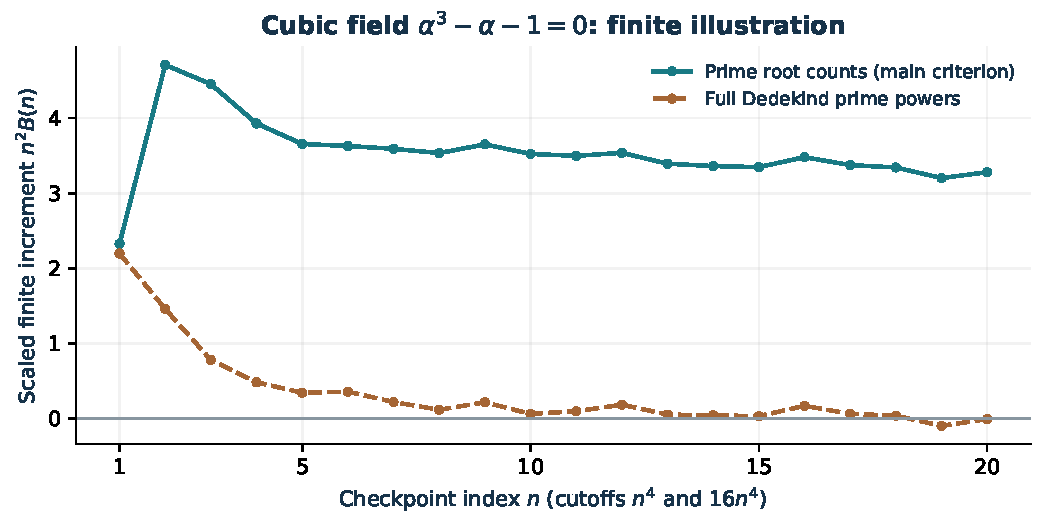
\includegraphics[width=.96\textwidth]{../figures/cubic_checkpoints.pdf}
\caption{Finite values of the scaled centering-free cubic statistic.
The displayed range neither proves nor disproves an eventual bound.
All arithmetic splitting decisions are exact; the weighted sums are
floating-point illustrations.}
\end{figure}

\subsection{The exact interpolation cost}

\begin{figure}[htbp]
\centering
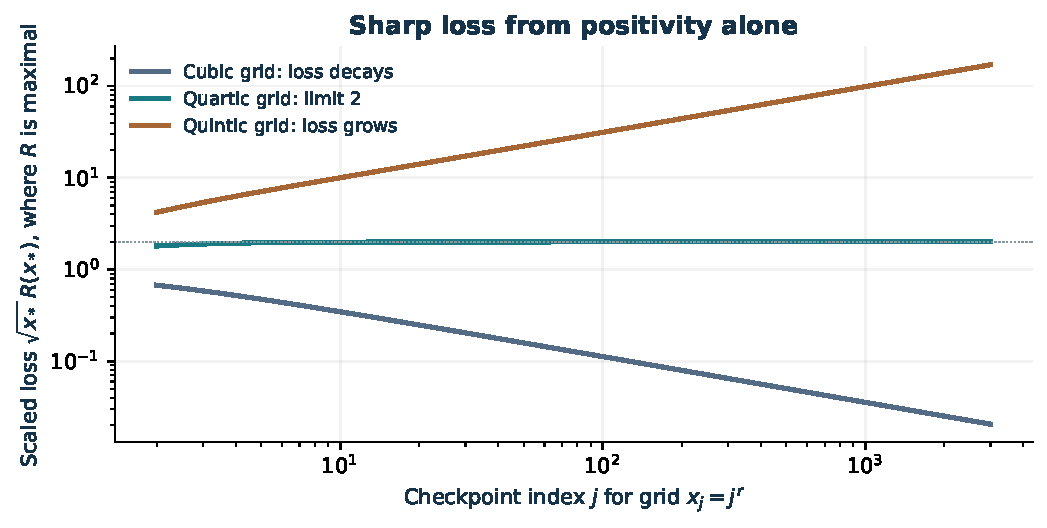
\includegraphics[width=.96\textwidth]{../figures/sampling_loss.pdf}
\caption{The extremal positive-measure construction from
Proposition~\ref{prop:sampling-sharp}. Although every sampled remainder
is zero, normalized peaks tend to zero for a cubic grid, tend to $2$
for a quartic grid, and grow for a quintic grid. This is a
positivity-only obstruction, not a counterexample for prime coefficients.}
\end{figure}

For each adjacent pair of checkpoints the exact worst loss is
$A\log S(r)$, with $S$ the Specht ratio. The formula and proof in this
report remove any numerical dependence from the interpolation theorem.
The plot is only a picture of the proved construction.\cite{specht}

\subsection{Reproduction commands and formalization status}

From the root of the unpacked archive, run:
\begin{verbatim}
python3 code/check_models.py
python3 code/check_source_blobs.py
python3 code/cubic_checkpoints.py --max-n 20
python3 code/make_figures.py
cd report
latexmk -pdf -interaction=nonstopmode -halt-on-error report.tex
\end{verbatim}

The mathematical check scripts require only the standard library.
The figure script additionally needs Matplotlib and NumPy. The report
uses a conventional pdfLaTeX installation. Selected unmodified upstream
source files, their licenses, and hashes are included for inspection.
The audit driver can optionally compare a complete separately obtained
checkout with the full recorded GitHub blob inventory.

\path{formalization/TransferInterfaces.lean} gives definitions for the
new target and elementary interfaces, with no claimed formal proof of
the new results. \path{formalization/Audit.lean} prints the exact types
and axioms of the upstream endpoints when run in the pinned project.
Neither file was compiled in this session. The complete archive is
intended to be reviewable and reproducible without confusing numerical
examples, human proofs, source extraction, and kernel verification.

\section{Conclusion}

The highest-value next research task is a new arithmetic realization of
the nonabelian root-count statistic. The existing analytic machinery can
already turn its square-root one-sided estimate into a theorem, and
the present report reduces the estimate to explicit finite sums on a
sparse sequence of scales. Fixed congruence approximation cannot create
the required nonlinear character information; this is now quantified
for arbitrary finite Galois groups.

The auxiliary Selmer machinery supplies a second route to investigate,
but its useful output is a family of controlled twists. A fixed-module
comparison is needed before small normalized lengths can prove
vanishing. The ramification-budget inequality makes that gap exact.
These are actionable mathematical boundaries and reusable deductions,
while the cubic RH estimate and the broader conjectures remain
unproved in this work.

\appendix
\section{Source map}

Paths below are relative to the pinned repository. The included files
are byte-for-byte copies, not a standalone compilable subset.
\begin{longtable}{@{}p{.59\textwidth}p{.36\textwidth}@{}}
\toprule
File & Relevance\\
\midrule
\endhead
\path{grh/src/Statements.lean}, \path{grh/src/Main.lean} & Exact exported theorem scope.\\[4pt]
\path{grh/src/New/Reduction/MainInequality.lean} & Matched determinant comparison and losses.\\[4pt]
\path{grh/src/New/Reduction/OneSidedBound.lean} & Arithmetic remainder estimate and the final nonvanishing theorem.\\[4pt]
\path{grh/src/New/Reduction/PrimeSums.lean} & Positive coefficients and congruence-sensitive place sums.\\[4pt]
\path{grh/src/New/Reduction/Zeros/Criterion.lean} & Auxiliary quadratic twists and pole detection.\\[4pt]
\path{grh/src/Lib/Analytic/Landau.lean} & One-sided meromorphic Laplace-transform argument.\\[4pt]
\path{grh/src/Lib/General/NumberTheory/PadicLimitsValuation.lean} & Normalized length.\\[4pt]
\path{grh/src/New/Congruences/Selmer/GeneralTheorem.lean} & Simultaneous powers, ramification, and Selmer budgets.\\[4pt]
\path{grh/src/New/Congruences/Selmer/Line.lean} & Coefficient-ring quantifiers and bounded-support construction.\\[4pt]
\path{grh/src/New/Congruences/Selmer/AuxiliaryPrimes.lean} & Nonempty tied-prime set.\\[4pt]
\path{grh/src/New/Congruences/FitTwistsExist.lean} & The per-prime/embedding twist selection used in the determinant proof.\\
\bottomrule
\end{longtable}

\begin{thebibliography}{99}
\bibitem{grh-readme} Luke Sernau and collaborators,
\emph{GRH for Dirichlet $L$-functions, in Lean 4}, readable-edition README,
commit \path{72fead102f663d5c7a407964a13dc0cf9d977207} (2026).
\url{https://github.com/lsernau/grh-lean/blob/72fead102f663d5c7a407964a13dc0cf9d977207/grh/README.md}.
\bibitem{grh-main} Same repository, \emph{Main.lean}.
\url{https://github.com/lsernau/grh-lean/blob/72fead102f663d5c7a407964a13dc0cf9d977207/grh/src/Main.lean}.
\bibitem{grh-statements} Same repository, \emph{Statements.lean}.
\url{https://github.com/lsernau/grh-lean/blob/72fead102f663d5c7a407964a13dc0cf9d977207/grh/src/Statements.lean}.
\bibitem{grh-guide} Same repository, \emph{Reading guide}.
\url{https://github.com/lsernau/grh-lean/blob/72fead102f663d5c7a407964a13dc0cf9d977207/grh/GUIDE.md}.
\bibitem{main-inequality} Same repository, \emph{The main inequality}.
\url{https://github.com/lsernau/grh-lean/blob/72fead102f663d5c7a407964a13dc0cf9d977207/grh/src/New/Reduction/MainInequality.lean}.
\bibitem{one-sided} Same repository, \emph{The one-sided bound}.
\url{https://github.com/lsernau/grh-lean/blob/72fead102f663d5c7a407964a13dc0cf9d977207/grh/src/New/Reduction/OneSidedBound.lean}.
\bibitem{prime-sums} Same repository, \emph{Prime sums}.
\url{https://github.com/lsernau/grh-lean/blob/72fead102f663d5c7a407964a13dc0cf9d977207/grh/src/New/Reduction/PrimeSums.lean}.
\bibitem{criterion} Same repository, \emph{The one-sided criterion}.
\url{https://github.com/lsernau/grh-lean/blob/72fead102f663d5c7a407964a13dc0cf9d977207/grh/src/New/Reduction/Zeros/Criterion.lean}.
\bibitem{milne} J. S. Milne, \emph{Class Field Theory}, course notes,
Chebotarev density theorem and global class field theory.
\url{https://www.jmilne.org/math/CourseNotes/CFTc.pdf}.
\bibitem{suzuki} Masatoshi Suzuki, \emph{On variants of Chebyshev's
conjecture}, arXiv:2411.07436; published in The Ramanujan Journal.
\url{https://arxiv.org/abs/2411.07436}.
\bibitem{grenie} Lo\"ic Greni\'e and Giuseppe Molteni,
\emph{Explicit smoothed prime ideals theorems under GRH},
arXiv:1312.4465.
\url{https://arxiv.org/abs/1312.4465}.
\bibitem{setiawan} Sandi Setiawan, \emph{The Primacohedron Trace
Formulation of the Riemann Hypothesis: A Guide to Reconstructing the
Alp\"oge--Claude Proof in Lean}, version 2, posted November 25, 2026.
Unrefereed preprint; cited for prior fourth-power sampling, not as an
independent arithmetic proof.
\url{https://www.preprints.org/manuscript/202611.0738}.
\bibitem{specht} Masaru Tominaga,
\emph{Specht's ratio and logarithmic mean in the Young inequality},
Mathematical Inequalities and Applications 7 (2004), 113--125.
\url{https://files.ele-math.com/abstracts/mia-07-13-abs.pdf}.
\bibitem{martin} Kimball Martin, \emph{Rationality fields of CM modular
forms}, arXiv:2509.24119.
\url{https://arxiv.org/abs/2509.24119}.
\bibitem{prior} Vladimir Reshetnikov, ProveIt incoming reports,
snapshot \path{13c30b3b677b691845466289bfdb792d11fefad5}.
Six archive identities are recorded in the accompanying provenance file.
\url{https://github.com/VladimirReshetnikov/ProveIt/tree/13c30b3b677b691845466289bfdb792d11fefad5/docs/incoming}.
\end{thebibliography}
\end{document}
